\documentclass{../TexTemplate/myslide}
\usepackage[slide,table,python]{../TexTemplate/mypackage}
\hypersetup{colorlinks=true,linkcolor=black,urlcolor=blue}
\usepackage{xcolor}

\lstset{language=tex,frame=none}

\renewcommand{\thefootnote}{\fnsymbol{footnote}}

\title[ToolsSeminar]{Tools Seminar}
\subtitle{Week 9 - Visualization}
\author[chhzh123]{Hongzheng~Chen}
\date[Mar 23, 2020]{Mar 23, 2020}

\begin{document}

\begin{frame}
\titlepage
\end{frame}

\begin{frame}
\tableofcontents
\end{frame}

\section{Overview}
\begin{frame}
\sectionpage
\end{frame}

\begin{frame}{Visualization\protect\footnote{Ref: \url{https://shellywhen.github.io/Visualization/Outline-Visualization.html\#slide=3}}}
Visualization is used to \textbf{gain or show insights through data}
\begin{itemize}
	\item Information visualization
	\begin{itemize}
		\item not only statistical charts; various visualization forms help to show multi-attributes, topological structure, and complex relationships
		\item actually it is a sub-topic of human-computer interaction (HCI) with top-tier conference \href{https://chi2020.acm.org/}{CHI}
		\item good visualizations help your paper to be accepted!
	\end{itemize}
	\item Scientific visualization
	\begin{itemize}
		\item a sub-topic of CG
		\item emphasizing on realistic renderings of volumes, surfaces, illumination sources, etc.
	\end{itemize}
\end{itemize}
We will focus on information visualization
\end{frame}

\begin{frame}{Catalog of Information visualization}
\begin{itemize}
	\item Tables
	\item Bar charts
	\item Flow charts
	\item Functions
	\item Graphs / Networks
	\item Time series
	\item Text
	\item Geo-spacial
	\item $\cdots$
\end{itemize}
\end{frame}

\begin{frame}{Tables}
The most commonly seen data type
\begin{center}
\begin{tabular}{cccc}\hline
 & Col 1 & Col 2 & Col 3\\\hline
Row 1 & & &\\
Row 2 & & &\\
Row 3 & & &\\\hline
\end{tabular}
\end{center}
Tools: Excel, \href{https://www.tableau.com/}{Tableau}, \LaTeX
\begin{itemize}
	\item One of the \href{https://awards.acm.org/about/2019-turing}{2019 Turing Award} Winners: Pat Hanrahan (Tableau cofounder)
\end{itemize}
\end{frame}

\begin{frame}{Bar Charts}
\begin{figure}
\centering
\includegraphics[width=\linewidth]{fig/bar_chart_eg.png}
\caption*{\small Fig source: Nathan Beckmann, Po-An Tsai, Daniel Sanchez, \emph{Scaling Distributed Cache Hierarchies through Computation and Data Co-Scheduling}, HPCA, 2015}
\end{figure}
Tools: \href{https://matplotlib.org/}{Matplotlib}, \href{https://plot.ly/}{Plotly}\\
* Pay attention to the figures when you read papers. There exists lots of details!
\end{frame}

\begin{frame}{Flow charts}
\begin{figure}
\centering
\includegraphics[width=\linewidth]{fig/flow_chart_eg.png}
\caption*{\small Fig source: Nathan Beckmann, Po-An Tsai, Daniel Sanchez, \emph{Scaling Distributed Cache Hierarchies through Computation and Data Co-Scheduling}, HPCA, 2015}
\end{figure}
Tools: \href{https://products.office.com/en-us/visio/flowchart-software}{Microsoft Visio} (\href{https://ms.sysu.edu.cn/}{enterprise version}), \href{https://www.draw.io/}{draw.io}
\end{frame}

\begin{frame}{Functions (2D \& 3D)}
\begin{columns}
\begin{column}{0.45\linewidth}
\begin{center}
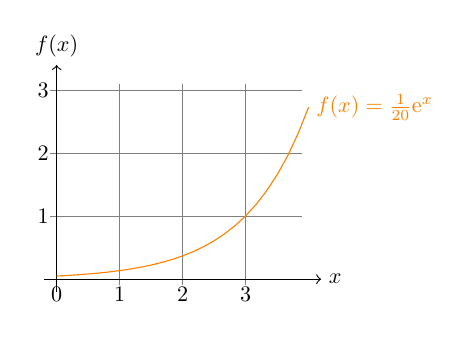
\begin{tikzpicture}[domain=0:4,scale=0.8, every node/.style={scale=0.8}]
\draw[very thin,color=gray] (-0.1,-0.1) grid (3.9,3.1);
\draw[->] (-0.2,0) -- (4.2,0) node[right] {$x$};
\draw[->] (0,-0.2) -- (0,3.4) node[above] {$f(x)$};
\draw[color=orange] plot (\x,{0.05*exp(\x)})
	node[right] {$f(x) = \frac{1}{20} \mathrm e^x$};
\node[below] at (0,0) {$0$};
\node[below] at (1,0) {$1$};
\node[below] at (2,0) {$2$};
\node[below] at (3,0) {$3$};
\node[left] at (0,1) {$1$};
\node[left] at (0,2) {$2$};
\node[left] at (0,3) {$3$};
\end{tikzpicture}
\end{center}
\end{column}
\begin{column}{0.55\linewidth}
\qquad\\
\bigskip
\begin{figure}
\centering
\includegraphics[width=\linewidth]{fig/gradient-descent.png}
\end{figure}
\end{column}
\end{columns}
\bigskip
Tools: \href{https://matplotlib.org/}{Matplotlib}, \href{https://www.wolfram.com/mathematica/}{Mathematica}, \LaTeX{} \href{http://www.texample.net/tikz/}{TikZ}
\end{frame}

\begin{frame}{Graphs/Networks}
\begin{figure}
\centering
\includegraphics[width=0.4\linewidth]{fig/network_graphs.png}
\caption*{\small Fig source: \url{https://digi.uga.edu/network-graphs/}}
\end{figure}
\begin{itemize}
	\item Node-link diagram, tree map, bubble chart
	\item Tools: \href{https://networkx.github.io/}{networkx}, \LaTeX{} \href{http://ctan.math.washington.edu/tex-archive/graphics/pgf/contrib/tikz-cd/tikz-cd-doc.pdf}{Tikzcd}, \LaTeX{} \href{http://mirrors.ibiblio.org/CTAN/graphics/pgf/contrib/forest/forest-doc.pdf}{forest}, \href{https://plot.ly/}{Plotly}
\end{itemize}
\end{frame}

\begin{frame}{Time Series}
\begin{figure}
\centering
\includegraphics[width=0.7\linewidth]{fig/Gantt_graph.png}
\end{figure}
\begin{itemize}
	\item Line graph / Bar charts
	\item Gantt Chart
	\item Heat Map: Check your \href{https://github.com/}{Github} contribution (
\end{itemize}
\end{frame}

\begin{frame}{Text}
\begin{figure}
\centering
\includegraphics[width=0.6\linewidth]{fig/word_cloud.png}
\end{figure}
Tools: \href{https://www.wordclouds.com/}{WordCloud}, \href{http://www.wordle.net/}{Wordle}, $\ldots$
\end{frame}

\section{Matplotlib}
\begin{frame}
\sectionpage
\end{frame}

\begin{frame}[fragile]{Matplotlib}
\href{https://matplotlib.org/index.html}{Matplotlib}: A Python 2D plotting library which produces publication quality figures in a variety of hardcopy formats and interactive environments across platforms\\
\bigskip
\verb'pip install matplotlib'
\begin{itemize}
	\item Use Anaconda to install since the figure will pop out as a graphical window
	\item If you use WSL, you need to install graphical support
	\item \textbf{Highly recommend} to use Jupyter Notebook no matter which OS you use
\end{itemize}
\bigskip
* See \verb'matplotlib.ipynb' for demos
\end{frame}

\section{Draw.io}
\begin{frame}
\sectionpage
\end{frame}

\begin{frame}{Draw.io}
\href{https://www.draw.io/}{Draw.io} is free online diagram software for making flowcharts, process diagrams, org charts, UML, ER and network diagrams
\begin{itemize}
	\item Web-based
	\item Open-sourced
	\item Support \LaTeX formulas
	\item Export as pdf files
\end{itemize}
\end{frame}

\section{TikZ}
\begin{frame}
\sectionpage
\end{frame}

\begin{frame}[fragile]{TikZ}
\href{http://www.texample.net/tikz/}{TikZ} and PGF are \TeX packages for creating graphics programmatically
\begin{itemize}
	\item If you have installed TeXLive completely, TikZ must has been installed
	\item Called by \verb'\usepackage{tikz}'
	\item Manual: \url{http://www.texample.net/media/pgf/builds/pgfmanualCVS2012-11-04.pdf}
	\item English tutorial from Overleaf: \url{https://www.overleaf.com/learn/latex/TikZ_package}
	\item Chinese tutorial: \url{https://www.latexstudio.net/archives/9774}
	\item Wiki book: \url{https://en.wikibooks.org/wiki/LaTeX/PGF/TikZ}
\end{itemize}
* \href{http://ctan.math.washington.edu/tex-archive/graphics/pgf/contrib/tikz-cd/tikz-cd-doc.pdf}{Tikz-cd}: commutative diagrams
\end{frame}

\begin{frame}[fragile]{TikZ Basis}
\begin{itemize}
	\item \verb'\begin{tikzpicture} ... \end{tikzpicture}'
	\item \verb'\node [attribute] (nodelabel) at (coordinate) {texts};'
	\item \verb'\draw (nodelabel) to (nodelabel);'
	\item Every command ends with \verb';'
\end{itemize}
\end{frame}

\begin{frame}[fragile]{TikZ Example}
\small
\begin{columns}
\begin{column}{0.4\linewidth}
\begin{center}
\begin{tikzpicture}
\node [left] (a) at (0,0) {$A$};
\node [right] (b) at (1,1) {$B$};
\draw [color=red!50,->] (a) -- (b);
\end{tikzpicture}
\end{center}
\begin{lstlisting}[basicstyle=\tiny]
\begin{tikzpicture}
\node [left] (a) at (0,0) {$A$};
\node [right] (b) at (1,1) {$B$};
\draw [color=red!50,->] (a) -- (b);
\end{tikzpicture}
\end{lstlisting}
\small * Use \verb'cycle' to draw closed curves
\end{column}
\begin{column}{0.6\linewidth}
\begin{center}
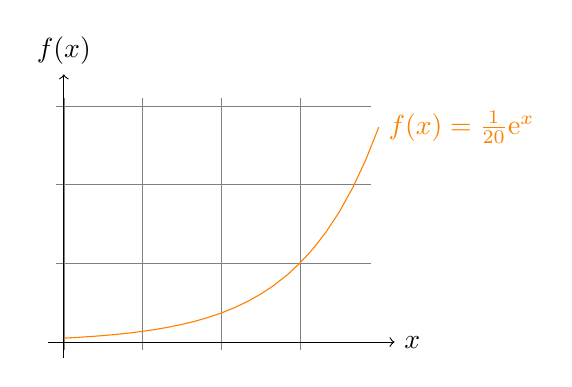
\begin{tikzpicture}[domain=0:4]
\draw[very thin,color=gray] (-0.1,-0.1) grid (3.9,3.1);
\draw[->] (-0.2,0) -- (4.2,0) node[right] {$x$};
\draw[->] (0,-0.2) -- (0,3.4) node[above] {$f(x)$};
\draw[color=orange] plot (\x,{0.05*exp(\x)})
	node[right] {$f(x) = \frac{1}{20} \mathrm e^x$};
\end{tikzpicture}
\end{center}
\begin{lstlisting}[basicstyle=\tiny]
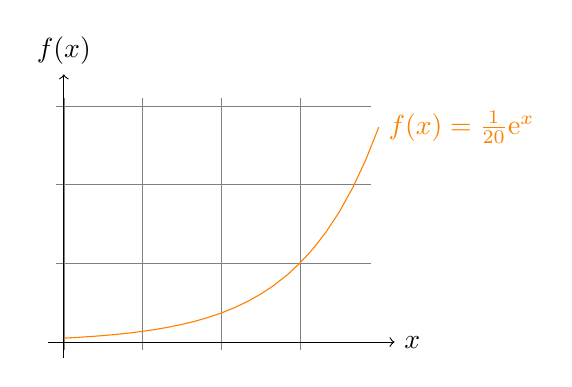
\begin{tikzpicture}[domain=0:4]
\draw[very thin,color=gray] (-0.1,-0.1) grid (3.9,3.1);
\draw[->] (-0.2,0) -- (4.2,0) node[right] {$x$};
\draw[->] (0,-0.2) -- (0,3.4) node[above] {$f(x)$};
\draw[color=orange] plot (\x,{0.05*exp(\x)})
	node[right] {$f(x) = \frac{1}{20} \mathrm e^x$};
\end{tikzpicture}
\end{lstlisting}
\end{column}
\end{columns}
\end{frame}

\begin{frame}[fragile]{Tree}
\begin{columns}
\begin{column}{0.5\linewidth}
\begin{center}
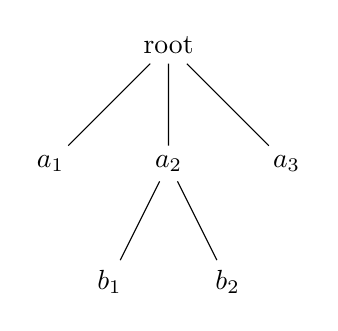
\begin{tikzpicture}
\node {root}
    child {node {$a_1$}}
    child {node {$a_2$}
        child {node {$b_1$}}
        child {node {$b_2$}}}
    child {node {$a_3$}};
\end{tikzpicture}
\end{center}
\begin{lstlisting}[basicstyle=\tiny]
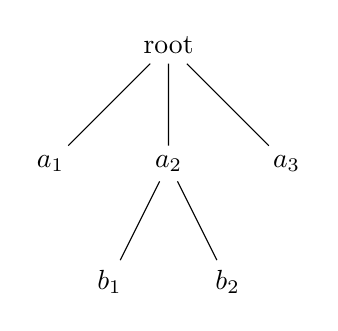
\begin{tikzpicture}
\node {root}
    child {node {$a_1$}}
    child {node {$a_2$}
        child {node {$b_1$}}
        child {node {$b_2$}}}
    child {node {$a_3$}};
\end{tikzpicture}
\end{lstlisting}
\end{column}
\begin{column}{0.5\linewidth}
\begin{tikzcd}[column sep=scriptsize]
& \text{root}\arrow[dash,dl]
  \arrow[dash,d]\arrow[dash,dr] & \\
a_1 & a_2\arrow[dash,dl]\arrow[dash,dr] & a_3\\
b_1 & & b_2
\end{tikzcd}
\begin{lstlisting}[basicstyle=\tiny]
\begin{tikzcd}[column sep=scriptsize]
& \text{root}\arrow[dash,dl]
  \arrow[dash,d]\arrow[dash,dr] & \\
a_1 & a_2\arrow[dash,dl]\arrow[dash,dr] & a_3\\
b_1 & & b_2
\end{tikzcd}
\end{lstlisting}
\end{column}
\end{columns}
\end{frame}

\begin{frame}[fragile]{Control Command (Loop)}
\begin{center}
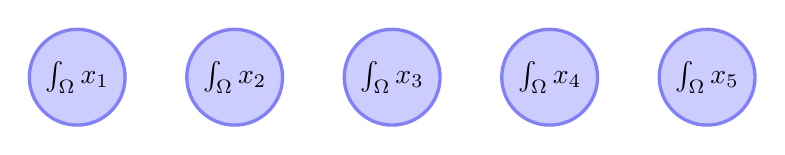
\begin{tikzpicture}
[L1Node/.style={circle,
    draw=blue!50, fill=blue!20, very thick,
    minimum size=10mm},
 L2Node/.style={rectangle,
    draw=green!50, fill=green!20, very thick,
    minimum size=10mm}]
\foreach \x in {1,...,5}
    \node[L1Node] (w1_\x) at (2*\x, 0){$\int_\Omega x_\x$};
\end{tikzpicture}
\end{center}
\begin{lstlisting}
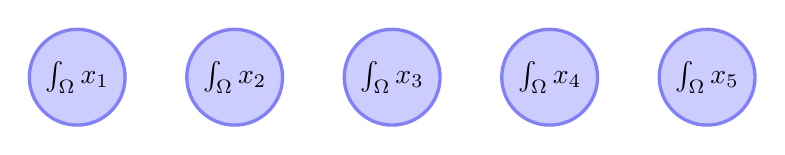
\begin{tikzpicture}
[L1Node/.style={circle,
    draw=blue!50, fill=blue!20, very thick,
    minimum size=10mm},
 L2Node/.style={rectangle,
    draw=green!50, fill=green!20, very thick,
    minimum size=10mm}]
\foreach \x in {1,...,5}
    \node[L1Node] (w1_\x) at (2*\x, 0){$\int_\Omega x_\x$};
\end{tikzpicture}
\end{lstlisting}
\end{frame}

\section{Summary}
\begin{frame}
\sectionpage
\end{frame}

\begin{frame}{Summary}
\begin{itemize}
	\item Overview
	\item Matplotlib
	\item Draw.io
	\item TikZ
\end{itemize}
\end{frame}

\end{document}